% 封面图：210mm x 168mm（与 ElegantBook 默认封面 1280x1024 同比例）
% 编译：xelatex cover.tex  ->  cover.pdf
\documentclass[tikz,border=0pt]{standalone}
\usepackage{tikz}
\usetikzlibrary{arrows.meta,positioning,calc,decorations.pathreplacing,
  decorations.markings,patterns,shadows.blur}
\usepackage{fontspec}
\setmainfont{Consolas}

\definecolor{navy}{RGB}{9,26,48}
\definecolor{navy2}{RGB}{16,48,86}
\definecolor{lineblue}{RGB}{52,120,190}
\definecolor{cyan}{RGB}{70,200,220}
\definecolor{amber}{RGB}{242,166,58}
\definecolor{soft}{RGB}{180,205,230}

\begin{document}
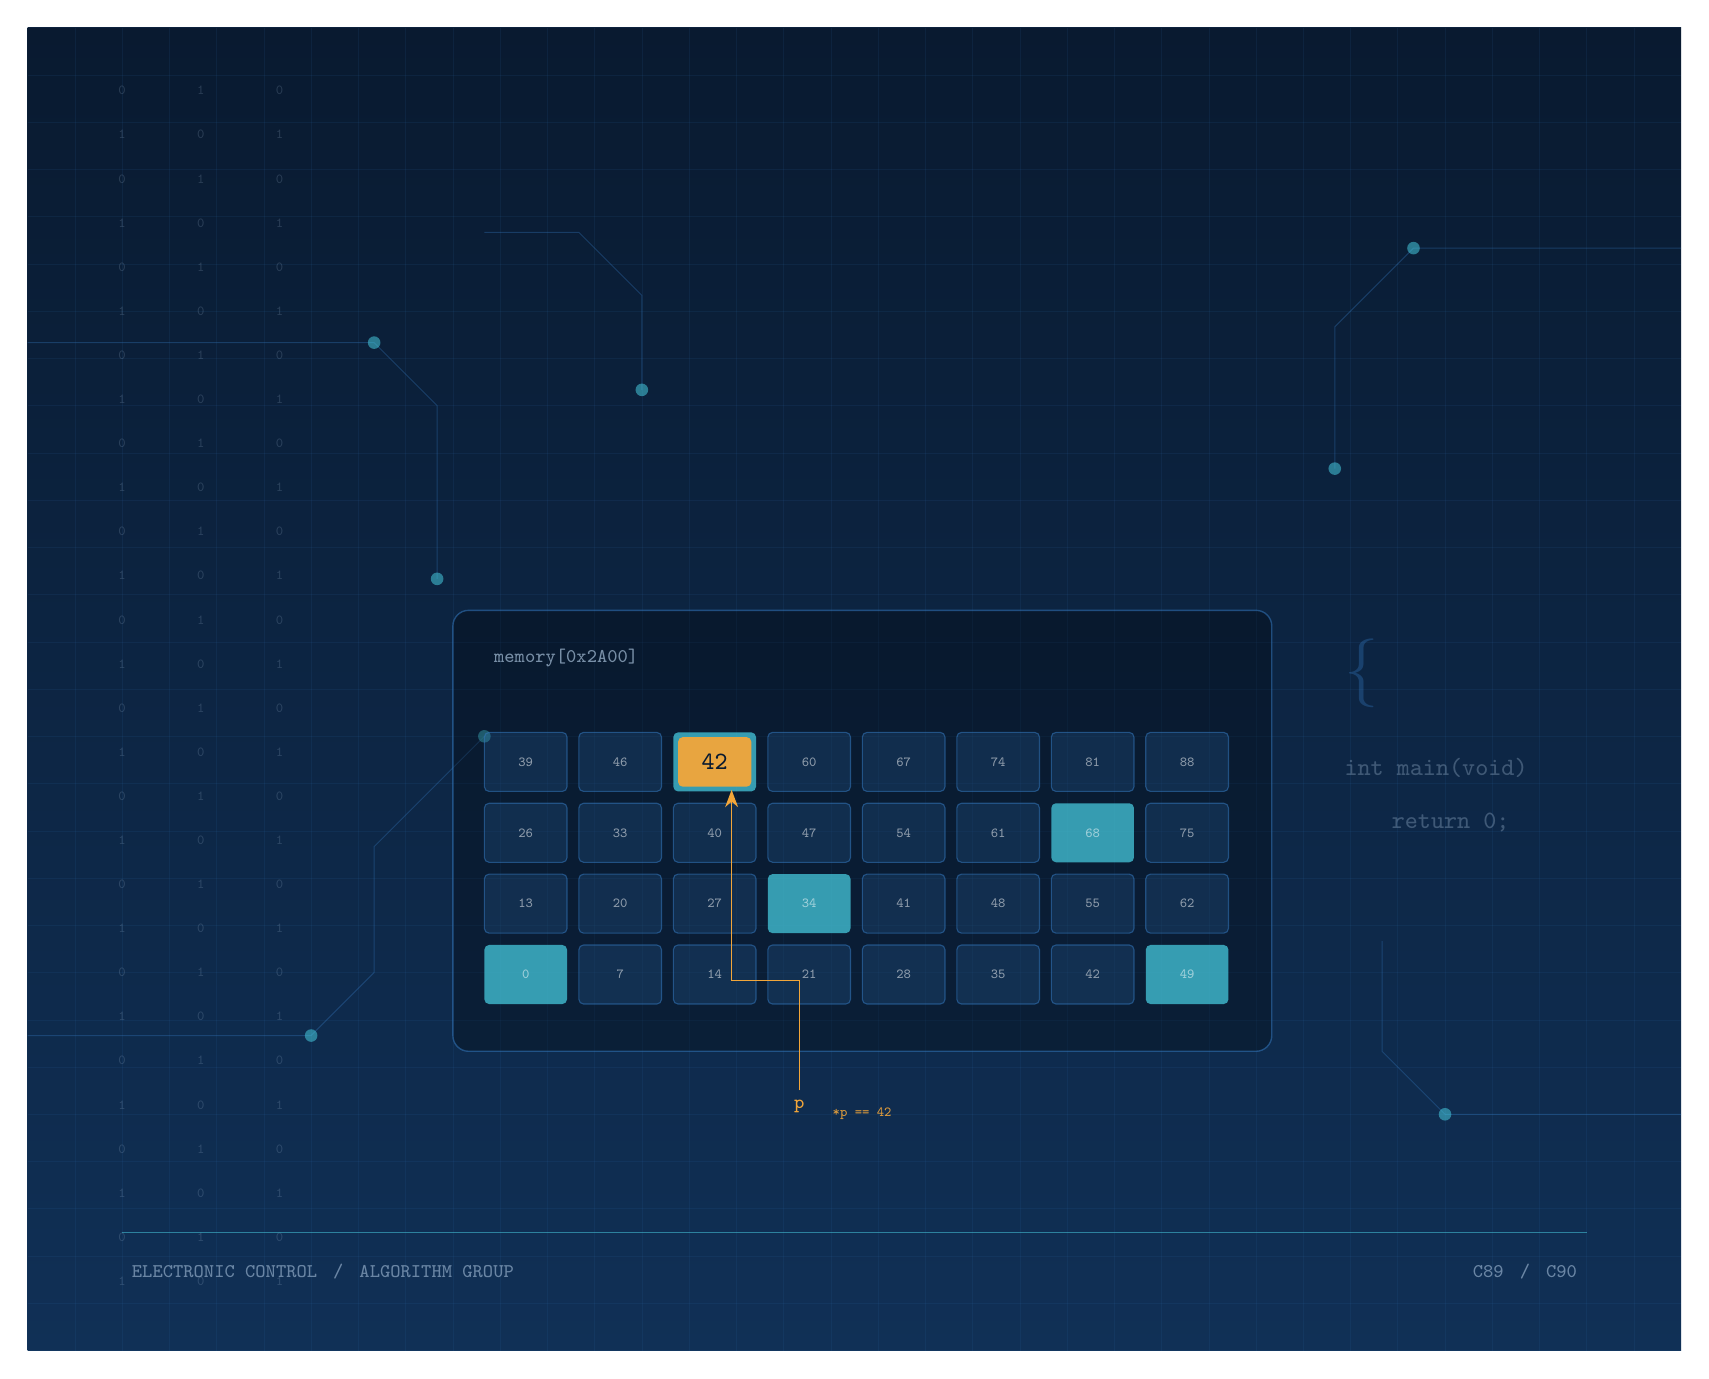
\begin{tikzpicture}[x=1mm,y=1mm]
  \clip (0,0) rectangle (210,168);

  % 背景渐变
  \shade[top color=navy, bottom color=navy2] (0,0) rectangle (210,168);

  % 细网格
  \foreach \x in {0,6,...,210} {
    \draw[lineblue,opacity=0.10,line width=0.2pt] (\x,0) -- (\x,168);
  }
  \foreach \y in {0,6,...,168} {
    \draw[lineblue,opacity=0.10,line width=0.2pt] (0,\y) -- (210,\y);
  }

  % 左侧二进制瀑布
  \foreach \col/\x in {0/12,1/22,2/32} {
    \foreach \row in {0,...,27} {
      \pgfmathparse{int(mod(\col*7+\row*3,2))}
      \ifnum\pgfmathresult=1
        \node[font=\ttfamily\tiny,text=soft,opacity=0.18]
          at (\x,160-\row*5.6) {1};
      \else
        \node[font=\ttfamily\tiny,text=soft,opacity=0.18]
          at (\x,160-\row*5.6) {0};
      \fi
    }
  }

  % 电路走线
  \begin{scope}[lineblue,opacity=0.35,line width=0.35pt]
    \draw (0,128) -- (44,128) -- (52,120) -- (52,98);
    \draw (0,40) -- (36,40) -- (44,48) -- (44,64) -- (58,78);
    \draw (210,140) -- (176,140) -- (166,130) -- (166,112);
    \draw (210,30) -- (180,30) -- (172,38) -- (172,52);
    \draw (58,142) -- (70,142) -- (78,134) -- (78,122);
  \end{scope}
  \foreach \p in {(44,128),(52,98),(36,40),(58,78),(176,140),(166,112),(180,30),(78,122)} {
    \fill[cyan,opacity=0.55] \p circle (0.8);
  }

  % 中央：内存条带 + 指针
  \begin{scope}[shift={(58,44)}]
    % 背板
    \fill[black,opacity=0.28,rounded corners=2mm] (-4,-6) rectangle (100,50);
    \draw[lineblue,opacity=0.55,rounded corners=2mm,line width=0.5pt]
      (-4,-6) rectangle (100,50);

    % 标题行
    \node[anchor=west,font=\ttfamily\scriptsize,text=soft,opacity=0.65]
      at (0,44) {memory[0x2A00]};

    % 8x4 内存单元
    \foreach \r in {0,...,3} {
      \foreach \c in {0,...,7} {
        \pgfmathparse{int(mod(\r*5+\c*3,7))}
        \ifnum\pgfmathresult=0
          \fill[cyan,opacity=0.75,rounded corners=0.6mm]
            ({\c*12},{\r*9}) rectangle ++(10.5,7.5);
        \else
          \fill[lineblue,opacity=0.20,rounded corners=0.6mm]
            ({\c*12},{\r*9}) rectangle ++(10.5,7.5);
          \draw[lineblue,opacity=0.55,rounded corners=0.6mm]
            ({\c*12},{\r*9}) rectangle ++(10.5,7.5);
        \fi
        \pgfmathtruncatemacro{\val}{int(mod(\r*13+\c*7,97))}
        \node[font=\ttfamily\tiny,text=white,opacity=0.52]
          at ({\c*12+5.25},{\r*9+3.75}) {\val};
      }
    }

    % 高亮单元与数值
    \fill[amber,opacity=0.95,rounded corners=0.6mm]
      (2*12+0.6,3*9+0.6) rectangle ++(9.3,6.3);
    \node[font=\ttfamily\small\bfseries,text=navy] at (2*12+5.25,3*9+3.75) {42};

    % 指针
    \node[font=\ttfamily\scriptsize,text=amber] (p) at (40,-13) {p};
    \draw[amber,line width=0.5pt,-{Stealth[length=2.2mm]}]
      (p.north) -- (40,3) -- (31.4,3) -- (31.4,27.2);
    \node[anchor=west,font=\ttfamily\tiny,text=amber,opacity=0.9]
      at (43,-14) {*p == 42};
  \end{scope}

  % 右侧大括号装饰
  \node[font=\ttfamily\Huge,text=lineblue,opacity=0.35,anchor=west]
    at (166,86) {\{};
  \node[font=\ttfamily\small,text=soft,opacity=0.30,anchor=west]
    at (166,74) {int main(void)};
  \node[font=\ttfamily\small,text=soft,opacity=0.30,anchor=west]
    at (172,67) {return 0;};

  % 底部信息
  \node[anchor=west,font=\ttfamily\scriptsize,text=soft,opacity=0.55]
    at (12,10) {ELECTRONIC CONTROL \;/\; ALGORITHM GROUP};
  \node[anchor=east,font=\ttfamily\scriptsize,text=soft,opacity=0.55]
    at (198,10) {C89 \;/\; C90};
  \draw[cyan,opacity=0.55,line width=0.4pt] (12,15) -- (198,15);
\end{tikzpicture}
\end{document}

